\chapter{Filters}

\begin{equation}
2\pi f=\omega
\end{equation}

\section{Parameters}

\centering
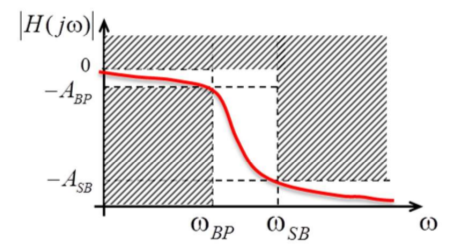
\includegraphics[width=0.5\textwidth]{mask.png}\\
\raggedright

Selectivity index
\begin{equation}
k=\frac{\omega_{BP}}{\omega_{SB}}
\end{equation}

Attenuation index
\begin{equation}
\varepsilon_{BP}=\sqrt{10^{A_{BP}/10}-1} \ \ \ \ \ \ \ \varepsilon_{BP}=\sqrt{10^{A_{SB}/10}-1}
\end{equation}

Discriminator factor 
\begin{equation}
k_{\varepsilon}=\frac{\varepsilon_{BP}}{\varepsilon_{SB}}<1
\end{equation}
Higher the attenuation in stop-band lower $k_{\varepsilon}$ is.

%------------------------------------------------------------------------%
\section{Butterworth Filters}
%------------------------------------------------------------------------%
Maximum flatness in passband.\\

General formula for the module 
\begin{equation}
|H(j\omega)|=\frac{1}{\sqrt{1+(\frac{\omega}{\Omega_0})^{2n}}}
\end{equation}
where n is the filter order.\\

To mach the in-band attenuation spec. we have to respect
\begin{equation}
\frac{\Omega_{BP}}{\Omega_0}\le \varepsilon_{BP}^{1/n}
\end{equation}

To mach the stop-band attenuation spec. we have to respect
\begin{equation}
\frac{\Omega_{SB}}{\Omega_0}\ge \varepsilon_{SB}^{1/n}
\end{equation}

So we get an interval of $\Omega_0$ and a formula for the filter order
\begin{equation}
\frac{\Omega_{BP}}{\varepsilon_{BP}^{1/n}} \ge \Omega_0 \le \frac{\Omega_{SB}}{\varepsilon_{SB}^{1/n}} \ \ \ \ \ \ \ \ \ \ \ \ \ \ n\ge \frac{\ln(k_{\varepsilon})}{\ln(k)}
\end{equation}

Poles in the Gauss plane are disposed as in figure


\centering
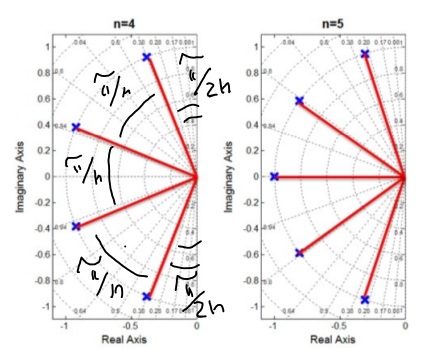
\includegraphics[width=0.35\textwidth]{Gaussbutt.png}\\
\raggedright

Table of Butterworth polynomials

\centering
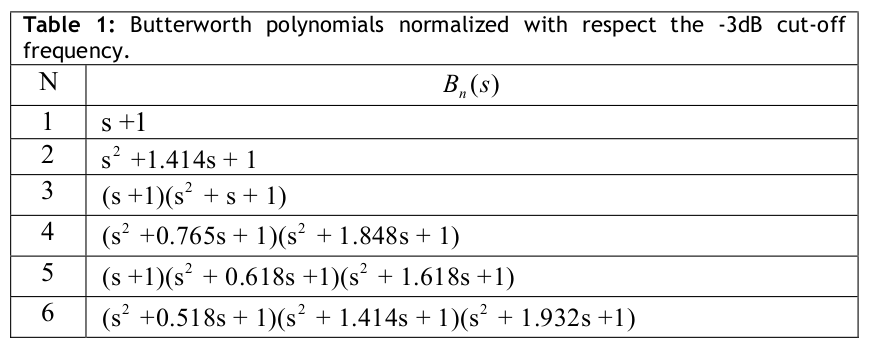
\includegraphics[width=0.5\textwidth]{butt.png}\\
\raggedright


%------------------------------------------------------------------------%
\section{Bessel Filters}
%------------------------------------------------------------------------%

Maximum phase linearity.\\
General formula for the module 
\begin{equation}
|H(s)|=J_n(0)/J_n(s)
\end{equation}
where n is the filter order.

Table of poles for a n order Bessel 

\centering
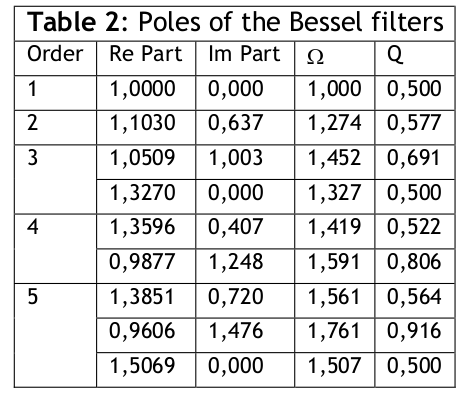
\includegraphics[width=0.35\textwidth]{bessel.png}\\
\raggedright

%------------------------------------------------------------------------%
\section{Chebyshev Type-I}
%------------------------------------------------------------------------%
Low number of poles good selectivity but bad phase.\\
General formula is
\begin{equation}
H(s)=\frac{K_n}{D_n(s)}
\end{equation}
where $D_n(s)$ are the Cheby. polynomials and $K_n$ is a coefficient to have $|H(0)|=1$ for filters of odd order and $|H(0)|=1/\sqrt{1+\varepsilon_{BP}^2}$ for even filters order (count the ripple).\\
\vspace{2mm}
Order of the filter form the specs can be derived as
\begin{equation}
n\ge \frac{arCosh(k_{\varepsilon}^{-1})}{arCosh(k^{-1})}
\end{equation} 

Poles derived from the following formulas to mach exactly the BP attenuation

\centering
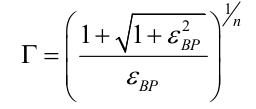
\includegraphics[width=0.15\textwidth]{gamma.png}\\
\raggedright


\centering
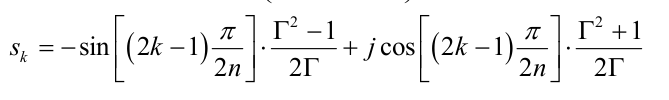
\includegraphics[width=0.45\textwidth]{s.png}\\
\raggedright

where we remember that 
\begin{equation}
\omega=\sqrt{r^2+i^2} \ \ \ \ \ \ \ Q=\frac{|omega|}{|2r|}
\end{equation}

Where k ranges form 1,2,...2n and only poles with negative real part have to be considered.\\

To mach SB attenuation exactly we have to use in $\Gamma$
\begin{equation}
\varepsilon_{BP}'=\frac{\varepsilon_{SB}}{Ch(n*arCh(1/k))}
\end{equation}


\centering
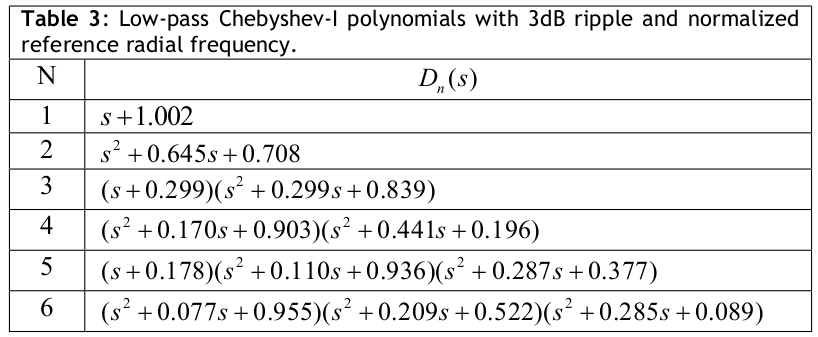
\includegraphics[width=0.5\textwidth]{cheby.png}\\
\raggedright

Poles in Gauss plane placed in an ellipse.\\





%------------------------------------------------------------------------%
%------------------------------------------------------------------------%
\section{Sallen-Key Cell}

\subsection{With K$>$1}
\centering
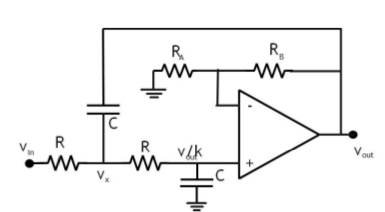
\includegraphics[width=0.35\textwidth]{skg.png}\\
\raggedright

With all R equal ,all capacitors equal C and K the gain of the amplifier 
\begin{equation}
\omega_0=\frac{1}{RC}\ \ \ \ \ \ \ \ \ \  \ \ \ \ \ \ \ \ Q=\frac{RC}{RC(k-1)+2RC}
\end{equation}
Form the Q equation we get the dependaces with k 
\begin{equation}
k=3-\frac{1}{Q} \ \ \ \ \ \ Q=\frac{1}{(3-k)}
\end{equation}
A variation of $\Delta k/k=\%$ is mapped in a Q variation of 

\begin{equation}
\Delta Q \simeq \Delta k \cdot Q^2
\end{equation}
The most significant change in the transfer function due to a change of Q is at the cut off frequency $\Omega_{bp}$; there we can define the proportion
\begin{equation}
10\% \ \ of \ \ \frac{\Delta Q}{Q} \propto 1dB
\end{equation}
Highes the Q bigger the variation for a given percentage bigger attenuation.\\


\subsection{With K=1}
\centering
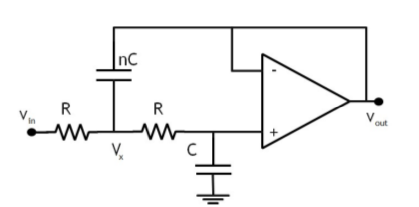
\includegraphics[width=0.35\textwidth]{skb.png}\\
\raggedright

With all R equal and K=1 the capacitor has to be different to add a degree of freedom to the system so
\begin{equation}
\omega_0=\frac{1}{\sqrt{n}RC}\ \ \ \ \ \ \ \ \ \ \ \ \ \ \ \ \ Q=\frac{\sqrt{n}}{2}
\end{equation}

\section{Non idealities}
When we get a non ideal op-amp with finite GBWP and DC gain and olso others poles or positive zeros this imperfections leads us to a change of Q like in the relations 
\begin{equation}
\frac{\Delta Q}{Q}\simeq 2Q\left(\frac{f_0}{GBWP}+\frac{f_0}{f_z}+\frac{f_0}{f_p}-\frac{1}{A_0}\right)
\end{equation}

%------------------------------------------------------------------------%
\section{Ladder}

From ladder networ first identify all variables V and I in the circuit 

\centering
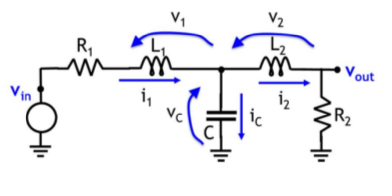
\includegraphics[width=0.35\textwidth]{ldd1.png}\\
\raggedright

Than make a flowgraph with all the integrations (with capacitor frmo current to voltage with inductors vice versa)

\centering
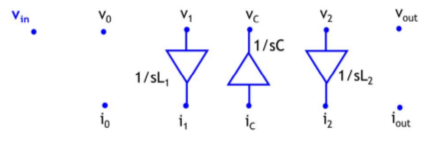
\includegraphics[width=0.5\textwidth]{ldd2.png}\\
\raggedright

Connect the nodes in order to have arrows directed in the amplifier ingresses and form the output of the amplifier to other variables

\centering
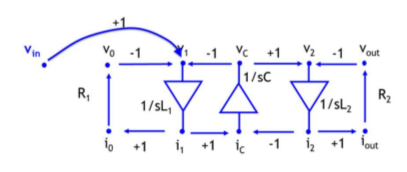
\includegraphics[width=0.5\textwidth]{ldd3.png}\\
\raggedright

Multiply all the current nodes by a factor $R^*$, all the branches from current to voltages by $1/R^*$ and all the branches form voltage to current by $R^*$. In this way we have only voltage signals like in figure below

\centering
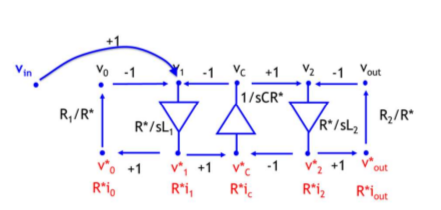
\includegraphics[width=0.5\textwidth]{ldd4.png}\\
\raggedright

In order to use virtual ground as current summing node we multiply by $1/R^*$ all the input nodes of the amplifiers in order to have current signals and for coherence we have to multiply by $R^*$ all opamps function.\\
Than since we will use inverting integrators we have to change sign at all the transfer functions and at all the inputs of the amplifiers

\centering
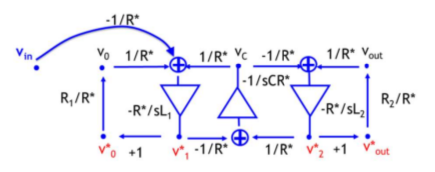
\includegraphics[width=0.5\textwidth]{ldd5.png}\\
\raggedright

Form this last scheme we get the filter implementation using integrators where 
\begin{equation}
C_1=L_1/R^{*2} \ \ \ \ \ \ \ \ \ \ \ \ \ \ C_2=L_2/R^{*2}  \ \ \ \ \ \ \ \ \ \ \ \ \ \ R_y=R^* \ \ \ \ \ \ \ \ \ \ \ \ R_x=\frac{R^{*2}}{R_2}-R^*
\end{equation}


\centering
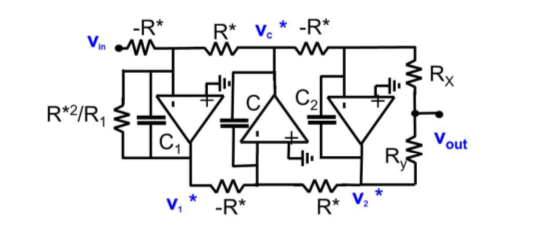
\includegraphics[width=0.5\textwidth]{ldd6.png}\\
\raggedright


The denormalization procedure changes the component values according to the following rules:

\begin{equation}
R_1=R_1^{(0)}M \ \ \ \ \ \ \ \ L_1=L_1^{(0)}M/N \ \ \ \ \ \ \ \ L_2=L_2^{(0)}M/N \ \ \ \ \ \ \ \ C=C^{(0)}/(MN) \ \ \ \ \ \ \ \ R_2=R_2^{(0)}M
\end{equation}

Where $N=2\pi f_0$ is the factor needed to get from 1rad/s to the desired $f_0$, the factor M is to rise the resistor values and $R^*$ is an additional degree of freedom.\\
Here we place $R=\alpha R^*$ and the two in-out resistor equal to R. Beacuse all resistor have to be positive we have a constrain on $R_x$ and from that a constrain on $\alpha$. Than we choose $\alpha $ and so we can choose olso the value of $R^*$ and from that M.\\
\vspace{5mm}
Transformation from LP to HP or BP in ladder implementation are 

\centering
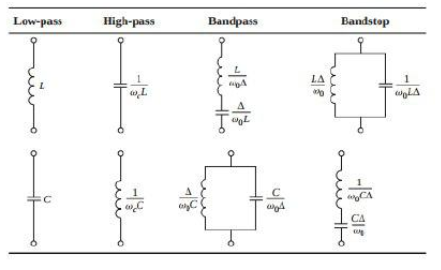
\includegraphics[width=0.8\textwidth]{ld.png}\\
\raggedright


\centering
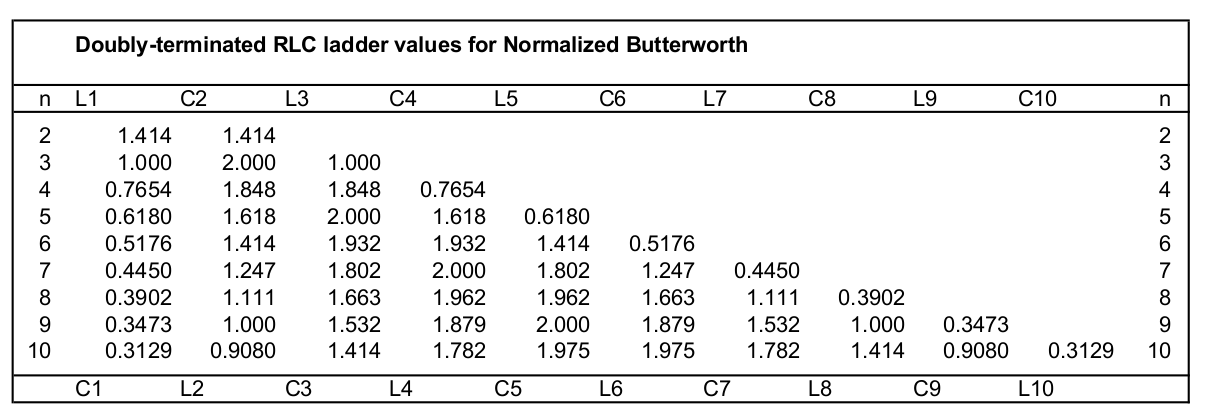
\includegraphics[width=0.9\textwidth]{ldb.png}\\
\raggedright


\centering
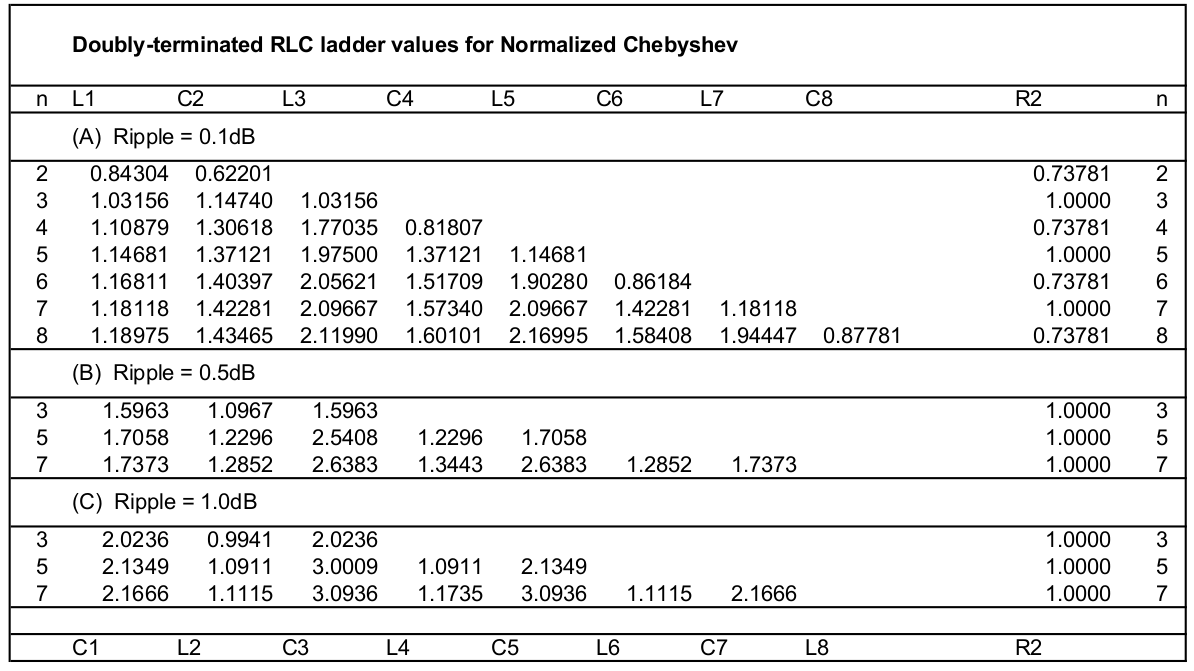
\includegraphics[width=0.9\textwidth]{ldc.png}\\
\raggedright

\centering
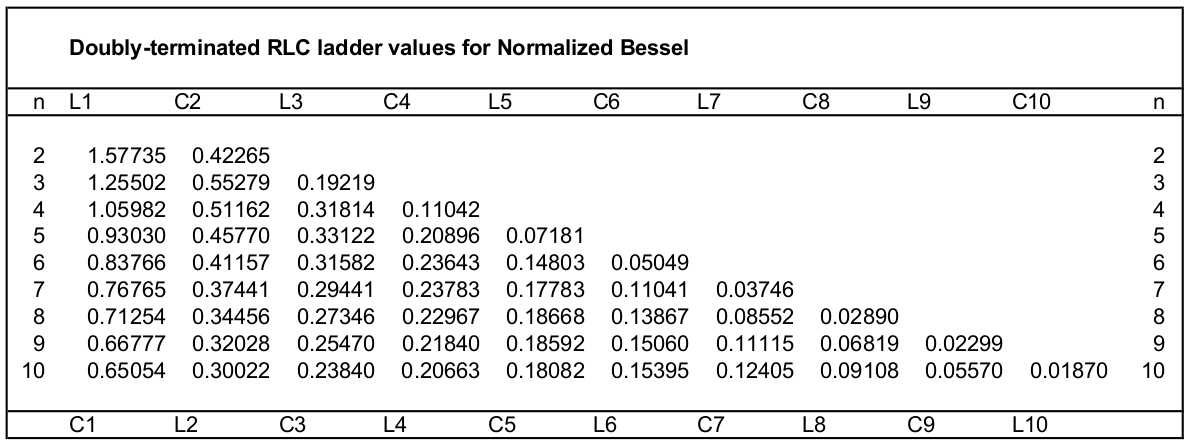
\includegraphics[width=0.9\textwidth]{ldb1.png}\\
\raggedright

